% vim: set tabstop=4:
% vim: set shiftwidth=4:
% vim: set expandtab:
\RHpresentationHead{
\documentclass[pdftex,unicode,xcolor=table]{beamer}
%\documentclass[pdftex,unicode,xcolor=table,notes=show]{beamer}
}

\RHarticleHead{
% This does not work, because of colors, \insertauthor, etc.
\documentclass[a4paper,12pt,pdftex,unicode]{article}
\usepackage[envcountsect]{beamerarticle}
}

\mode<presentation> {
    \usetheme{RedHat}
    \setbeamertemplate{navigation symbols}{}
    \setbeamercovered{transparent=5}
}
\mode<article> {
    \usepackage{fullpage}
}
\mode<handout> {
    \usepackage{pgfpages}
    \pgfpagesuselayout{4 on 1}[a4paper,landscape,border shrink=5mm]
}

\usepackage{beamerredhat}
\usepackage{etex}
\usepackage[utf8]{inputenc}
%\usepackage{czech}
\usepackage[czech]{babel}
\usepackage{setspace,amsfonts,calc,upquote,hyperref,floatflt,graphicx}
\usepackage[table]{xcolor}
\usepackage{colortbl}
\usepackage[absolute,overlay]{textpos}\textposquirk


% presentation title/author/etc.
\title{Improved Integration of SSSD and SUDO}
\institute{Michal Šrubař}
\date{}

% fancy section/part pages?
\fancySectionOpens
\fancyPartOpens

\begin{document}

% title pages
\mode<article> {
    \maketitle
    \newpage
}

% table of contents
%\mode<article> {
%    \newpage
%    \tableofcontents
%    \newpage
%}

\mode<presentation> {
    \begin{rhbg}
    \begin{frame}
        \titlepage
    \end{frame}
    \end{rhbg}
}

\begin{frame}
    \frametitle{SUDO}
    \begin{itemize}
        \item allows a user to execute a command as a different user
        \item SUDOers in \textit{/etc/sudoers}
        \item SUDOers in LDAP
    \end{itemize}
\end{frame}

\begin{frame}
    \frametitle{FreeIPA}
    \begin{itemize}
        \item what is it?
        \item benefits of having SUDOers in FreeIPA
    \end{itemize}
\end{frame}

\begin{frame}
    \frametitle{SSSD}
    \begin{itemize}
        \item popsat vyhody
    \end{itemize}
\end{frame}

\begin{frame}[fragile]
    \frametitle{Příklad uživatele v LDAPu}
        \begin{exampleblock}{uživatel v \texttt{/etc/passwd}}
\begin{verbatim}
jakub:x:500:500:Jakub Hrozek:/home/jakub:/bin/bash
\end{verbatim}
        \end{exampleblock}
        \begin{exampleblock}{uživatel v LDAPu}
\begin{verbatim}
dn: cn=jakub,ou=People,dc=redhat,dc=com
objectClass: posixAccount
objectClass: inetOrgPerson
uid: jakub
uidNumber: 500
gidNumber: 500
homeDirectory: /home/jakub
gecos: Jakub Hrozek
loginShell: /bin/bash
cn: jakub
\end{verbatim}
        \end{exampleblock}
\end{frame}

\begin{frame}
    \frametitle{Obecné centralizované řešení}
    \begin{itemize}
        \item Open Source komponenty existují a používají se
        \item složitá integrace, špatná abstrakce
        \begin{itemize}
            \item administrátor chce \textit{přidat uživatele}, ne
            \textit{vytvořit záznam v LDAPu}
        \end{itemize}
        \item hotová řešení většinou proprietární
        \begin{itemize}
            \item MS Active Directory
            \item Novell eDirectory
        \end{itemize}
    \end{itemize}
\end{frame}

\section{FreeIPA}
\begin{frame}
    \frametitle{FreeIPA}
    \begin{itemize}
        \item Free Identity, Policy, Audit
        \begin{itemize}
            \item Identity - správá uživatelů, strojů, služeb, DNS
            \item Policy - kvalita hesel, SUDO, HBAC
            \item Audit - TBD
        \end{itemize}
        \item cílem je jednoduchá instalace a správa
        \item existující Open Source komponenty
        \begin{itemize}
            \item LDAP - 389DS
            \item Kerberos - MIT Kerberos
            \item DNS - Bind
            \item CA - Red Hat Certificate Server
        \end{itemize}
        \item FreeIPA 2.0 - Fedora 15, RHEL 6.1
    \end{itemize}
\end{frame}

\begin{frame}[fragile]
    \frametitle{Příklad použití FreeIPA (v2)}
    \begin{exampleblock}{Instalace}
\begin{verbatim}
# ipa-server-install
\end{verbatim}
    \end{exampleblock}

    \begin{exampleblock}{Administrace - přidání uživatele}
\begin{verbatim}
# kinit admin
Password for admin@EXAMPLE.COM:
# ipa user-add -f John -l Doe jdoe
\end{verbatim}
    \end{exampleblock}
\end{frame}

\begin{frame}
    \frametitle{FreeIPA WebUI}
    \begin{figure}
        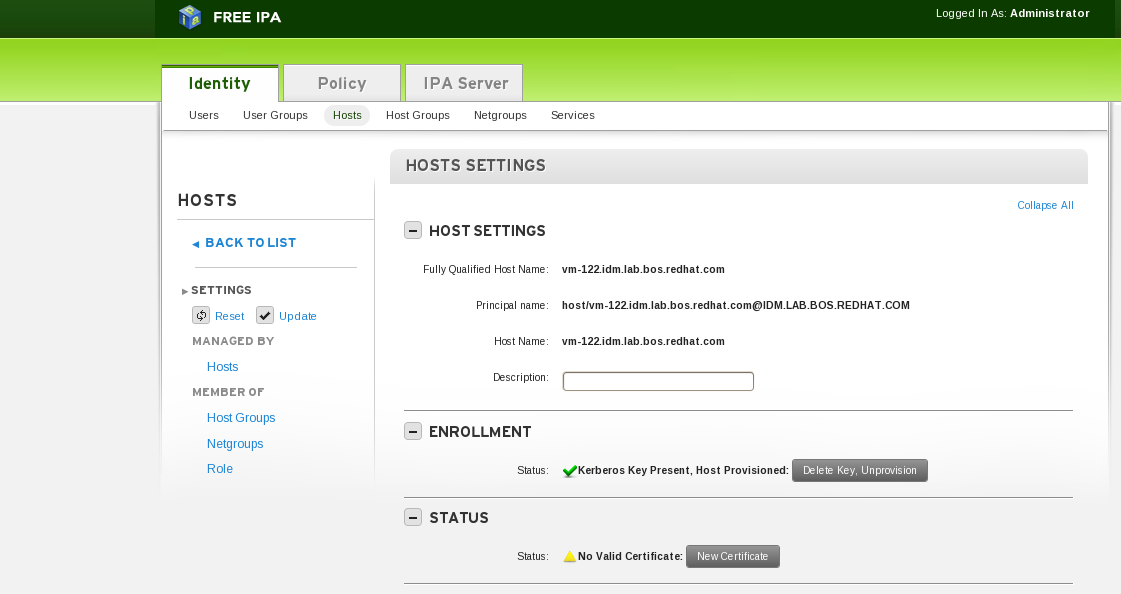
\includegraphics[scale=0.28]{img/ipa-webui.png}
    \end{figure}
\end{frame}

\section{SSSD}
\begin{frame}
    \frametitle{SSSD}
    \begin{itemize}
        \item klientská část centralizovaného řešení
        \item unixový démon, který běží na každém stroji v sítí
        \item poskytuje informace o uživateli z centrální databáze
        \item umožňuje uživateli se přihlásit
    \end{itemize}
    \begin{figure}
        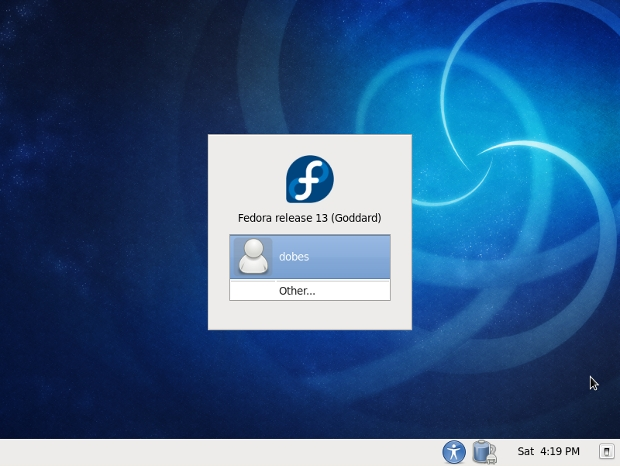
\includegraphics[scale=0.25]{img/gdm.png}
    \end{figure}
\end{frame}

\begin{frame}
    \frametitle{SSSD}
    \begin{itemize}
        \item binární balíčky k dispozici ve Fedoře, RHEL6, Ubuntu, OpenSuse, Gentoo, Debianu
        \item v současnosti podporuje SSSD několik typů serverů
        \begin{itemize}
            \item LDAP
            \item LDAP+Kerberos
            \item FreeIPA
            \item Active Directory (jako kombinaci LDAP+Kerberos)
        \end{itemize}
    \end{itemize}
\end{frame}

\begin{frame}[fragile]
    \frametitle{Výhody SSSD}
    \begin{itemize}
        \item podporuje více "domén"
        \begin{itemize}
            \item oddělené servery poskytující různá data
        \end{itemize}
        \item podpora více serverů pro jednu doménu
        \begin{itemize}
            \item redundance
        \end{itemize}
        \item detekce nedostupnosti a opětovné dostupnosti serveru
        \item cachování informací o uživatelích, případně hesel
        \begin{itemize}
            \item do cache se ukládají pouze opravdu použitá data
            \item není třeba kvůli každému dotazu zatěžovat server
            \item funguje i při nedostupném serveru
            \item záznamy v cache mohou postupně expirovat
            \item pro přihlášení se vždy snaží komunikovat se serverem (oproti \texttt{pam\_ccache})
        \end{itemize}
        \item pro některé druhy serverů specializované funkce
    \end{itemize}
\end{frame}

\section{Identity Management v Brně}
\begin{frame}
    \frametitle{FreeIPA v Brně}
    \begin{itemize}
        \item 4 stálí vývojáři + intern
        \begin{itemize}
            \item jedno volné místo
        \end{itemize}
        \item zbytek týmu v USA, Německu
        \item možnost spolupráce formou studentských prací
    \end{itemize}
\end{frame}

\begin{frame}
    \frametitle{Zapojte se do vývoje}
    \begin{itemize}
    \item home page - \url{www.freeipa.org}
        \begin{itemize}
        \item dokumentace, tarbally, zdrojovový kód
        \end{itemize}
    \item \url{http://fedorahosted.org/sssd}
        \begin{itemize}
            \item HOWTO, bugtracker
            \item v tarballu manuálové stránky, komentovaný sssd.conf
        \end{itemize}
    \item komunikace
        \begin{itemize}
        \item IRC - FreeNode, kanál \texttt{\#freeipa}
        \item konference \texttt{freeipa-\{devel,users,interest\}@redhat.com},
                         \texttt{sssd-devel@lists.fedorahosted.org}
        \end{itemize}
    \item hack on FreeIPA
        \begin{itemize}
        \item \url{http://freeipa.org/page/Contribute}
        \end{itemize}
    \end{itemize}
\end{frame}

\begin{frame}
    \frametitle{Děkuji za pozornost}
    \begin{itemize}
        \item Otázky?
    \end{itemize}
\end{frame}

\end{document}

